\documentclass[final,hyperref={pdfpagelabels=false}]{beamer}
\mode<presentation>
  {
    \usetheme{Berlin}
  \usetheme{Dreuw}
  }
  \usepackage{times}
  \usepackage{amsmath,amsthm, amssymb, latexsym}
  \boldmath
  \usepackage[english]{babel}
  \usepackage[latin1]{inputenc}
  \usepackage[orientation=portrait,size=a0,scale=1.4,debug]{beamerposter}

  %%%%%%%%%%%%%%%%%%%%%%%%%%%%%%%%%%%%%%%%%%%%%%%%%%%%%%%%%%%%%%%%%%%%%%%%%%%%%%%%%5
  \graphicspath{{figures/}}
  \title[Fancy Posters]{Software Development Methodologies }
  \author[Ivan Burke]{Cyber Defence Research Group}
  \institute[Council for Scientific and Industrial Research]{Defence, Peace, Safety and Security, \textit{Council for Scientific and Industrial Research}}
  \date{\today}


  %%%%%%%%%%%%%%%%%%%%%%%%%%%%%%%%%%%%%%%%%%%%%%%%%%%%%%%%%%%%%%%%%%%%%%%%%%%%%%%%%5
  \begin{document}
  \begin{frame}{ Waterfall Model} 
    %\vfill
   
    %\vfill
    \begin{block}{\large Description}
        %\centering
        The waterfall model is the classical model of software
        engineering. This model is one of the oldest models and is
        widely used in government projects and in many major
        companies. As this model emphasizes planning in early
        stages, it ensures design flaws before they develop. In
        addition, its intensive document and planning make it
        work well for projects in which quality control is a major
        concern.
        
        The pure waterfall life cycle consists of several non overlapping
        stages, as shown in the following figure. The
        model begins with establishing system requirements and
        software requirements and continues with architectural
        design, detailed design, coding, testing, and maintenance.
        The waterfall model serves as a baseline for many other
        life cycle models.
    \end{block}
     \begin{block}{\large Waterfall Model Diagram}
      \centering
        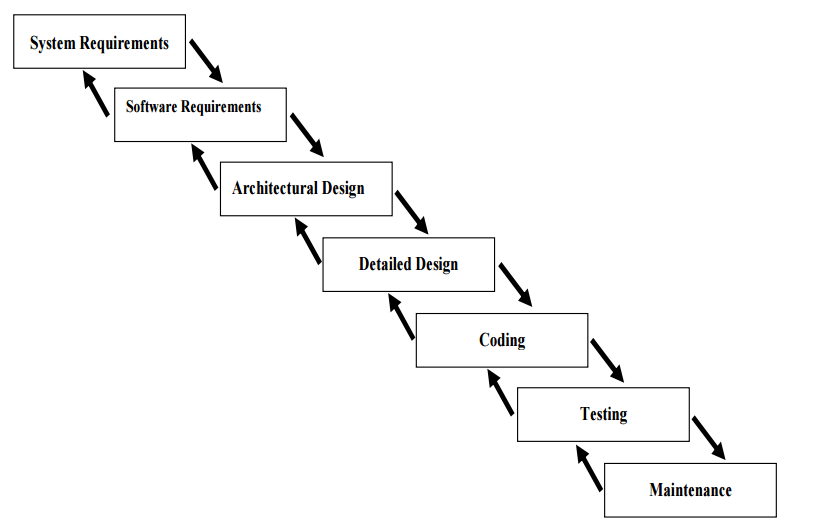
\includegraphics[width=.5\linewidth]{waterfall}
    \end{block}
    \vfill
    \begin{block}{\large Waterfall Model Steps}
        \begin{itemize}
            \item \textbf{ System requirements:} Establishes the components
                for building the system, including the hardware
                requirements, software tools, and other necessary
                components. Examples include decisions on
                hardware, such as plug-in boards (number of
                channels, acquisition speed, and so on), and decisions
                on external pieces of software, such as databases or
                libraries.
            \item \textbf{ Software requirements:} Establishes the expectations
                for software functionality and identifies which system
                requirements the software affects. Requirements
                analysis includes determining interaction needed with
                other applications and databases, performance
                requirements, user interface requirements, and so on.
            \item \textbf{ Architectural design:} Determines the software
                framework of a system to meet the specific
                requirements. This design defines the major
                components and the interaction of those components,
                but it does not define the structure of each
                component. The external interfaces and tools used in
                the project can be determined by the designer.
            \item \textbf{ Detailed design:} Examines the software components
                defined in the architectural design stage and produces
                a specification for how each component is
                implemented.
            \item \textbf{ Coding:} Implements the detailed design
                specification.
            \item \textbf{ Testing:} Determines whether the software meets the
                specified requirements and finds any errors present in
                the code.
            \item \textbf{ Maintenance:} Addresses problems and enhancement
                requests after the software releases.
        \end{itemize}
        
    \end{block}
    \vfill
    \begin{columns}[t]
      \begin{column}{.48\linewidth}
        \begin{block}{Advantages}
          \begin{itemize}
          \item Easy to understand and implement.
          \item Widely used and known (in theory!).
          \item Reinforces good habits: define-before- design,
                design-before-code.
          \item Identifies deliverables and milestones.
          \item Document driven, URD, SRD, … etc. Published
                documentation standards.
          \item Works well on mature products and weak teams.
          \end{itemize}
        \end{block}
        \vfill
        \begin{block}{Strengths}
          \begin{itemize}
          \item Minimizes planning
                overhead since it can
                be done up front.
          \item Structure minimizes
                wasted effort, so it
                works well for
                technically weak or
                inexperienced staff.
          \end{itemize}
        \end{block}
      \end{column}
      \begin{column}{.48\linewidth}
        \begin{block}{Disadvantages}
          \begin{itemize}
          \item Idealized, doesn't match reality well.
          \item Doesn't reflect iterative nature of exploratory
                development.
          \item Unrealistic to expect accurate requirements so
                early in project.
          \item Software is delivered late in project, delays discovery
                of serious errors.
          \item Difficult to integrate risk management.
          \item Difficult and expensive to make changes to
                documents, swimming upstream.
          \item Significant administrative overhead, costly for small
                teams and projects
          \end{itemize}
        \end{block}
        \begin{block}{Weaknesses}
          \begin{itemize}
          \item Inflexible
          \item Only the final phase
                produces a non documentation
                deliverable.
          \item Backing up to
                address mistakes is
                difficult.
          \end{itemize}
        \end{block}
      \end{column}
    \end{columns}
  \end{frame}
  \begin{frame}{Extreme Programing}
     \begin{block}{\large Description}
        \centering
        An approach to development, based on the development
        and delivery of very small increments of functionality. It
        relies on constant code improvement, user involvement in
        the development team and pair wise programming . It can
        be difficult to keep the interest of customers who are
        involved in the process. Team members may be unsuited
        to the intense involvement that characterizes agile
        methods. Prioritizing changes can be difficult where there
        are multiple stakeholders. Maintaining simplicity requires
        extra work. Contracts may be a problem as with other
        approaches to iterative development.
    \end{block}
    \vfill
    \begin{block}{\large  Extreme Programming Release Cycle}
      \centering
      
        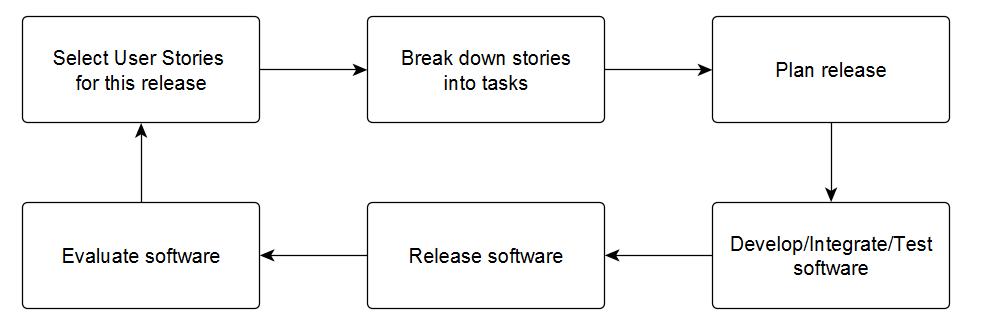
\includegraphics[width=.5\linewidth]{XP}
       
    \end{block}
    \vfill
    \begin{block}{\large Extreme Programming Practices}
        \centering
        \begin{itemize}
            \item \textbf{ Incremental planning:} Requirements are recorded on
            Story Cards and the Stories to be included in a release are
            determined by the time available and their relative priority.
            The developers break these stories into development
            "Tasks".
            \item \textbf{ Small Releases:} The minimal useful set of functionality
            that provides business value is developed first. Releases of
            the system are frequent and incrementally add
            functionality to the first release.
            \item \textbf{ Simple Design:} Enough design is carried out to meet the
            current requirements and no more.
            \item \textbf{ Test first development:} An automated unit test
            framework is used to write tests for a new piece of
            functionality before functionality itself is implemented.
            \item \textbf{ Refactoring:} All developers are expected to re-factor the
            code continuously as soon as possible code improvements
            are found. This keeps the code simple and maintainable.
            Pair Programming: Developers work in pairs, checking
            each other’s work and providing support to do a good job.
            \item \textbf{ Collective Ownership:} The pairs of developers work on
            all areas of the system, so that no islands of expertise
            develop and all the developers own all the code. Anyone
            can change anything.
            \item \textbf{ Continuous Integration:} As soon as work on a task is
            complete, it is integrated into the whole system. After any
            such integration, all the unit tests in the system must pass.
            \item \textbf{ Sustainable pace:} Large amounts of over-time are not
            considered acceptable as the net effect is often to reduce
            code quality and medium term productivity.
            \item \textbf{ On-site Customer:} A representative of the end-user of the
            system (the Customer) should be available full time for the
            use of the XP team. In an extreme programming process,
            the customer is a member of the development team and is
            responsible for bringing system requirements to the team
            for implementation.
        \end{itemize}
    \end{block}  
    \vfill
     \begin{block}{\large Extreme Programming Principles}
        \centering
        \begin{itemize}
            \item Incremental development is supported through small,
            frequent system releases.
            \item Customer involvement means full-time customer
            engagement with the team.
            \item People not process through pair programming,
            collective ownership and a process that avoids long
            working hours.
            \item Change supported through regular system releases.
            \item Maintaining simplicity through constant refactoring of
            code
        \end{itemize}
    \end{block}  
    \begin{columns}[t]
      \begin{column}{.48\linewidth}
        \begin{block}{Advantages}
          \begin{itemize}
          \item Lightweight methods suit small-medium size projects.
          \item Produces good team cohesion.
          \item Emphasises final product.
          \item Iterative.
          \item Test based approach to requirements and quality
                assurance.
          \end{itemize}
        \end{block}
        \vfill
      \end{column}
      \begin{column}{.48\linewidth}
        \begin{block}{Disadvantages}
          \begin{itemize}
          \item Difficult to scale up to large projects where
                documentation is essential.
          \item Needs experience and skill if not to degenerate into
                code-and-fix.
          \item Programming pairs is costly.
          \item Test case construction is a difficult and specialized
                skill
          \end{itemize}
        \end{block}
      \end{column}
    \end{columns}
  \end{frame} 
  
  \begin{frame}{Spiral}
        \begin{block}{\large Description}
            \centering
            The spiral model is similar to the incremental model, with
            more emphases placed on risk analysis. The spiral model
            has four phases: Planning, Risk Analysis, Engineering and
            Evaluation. A software project repeatedly passes through
            these phases in iterations (called Spirals in this
            model). The baseline spiral, starting in the planning
            phase, requirements are gathered and risk is
            assessed. Each subsequent spiral builds on the baseline
            spiral. Requirements are gathered during the planning
            phase. In the risk analysis phase, a process is undertaken
            to identify risk and alternate solutions. A prototype is
            produced at the end of the risk analysis phase. Software is
            produced in the engineering phase, along with testing at
            the end of the phase. The evaluation phase allows the
            customer to evaluate the output of the project to date
            before the project continues to the next spiral.
            
            In the spiral model, the angular component represents
            progress, and the radius of the spiral represents cost.
        \end{block}
        \vfill
    \begin{block}{\large Spiral Model}
      \centering
      
        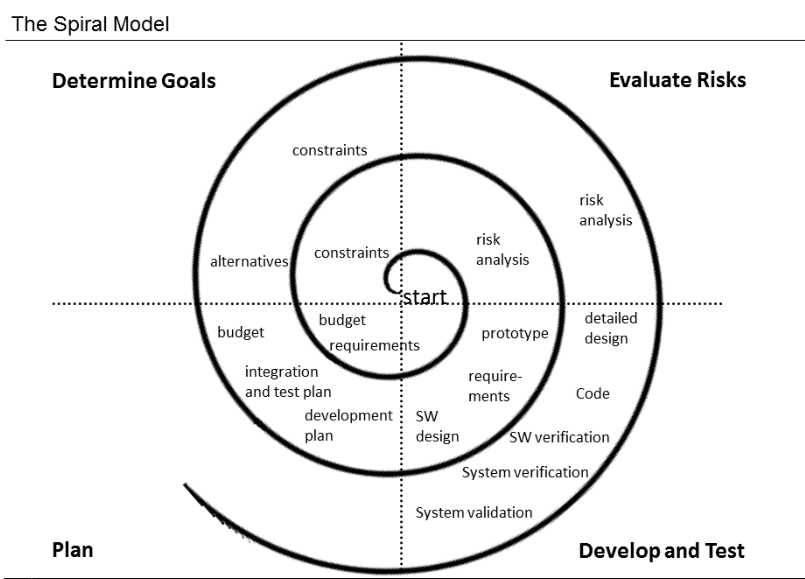
\includegraphics[width=.5\linewidth]{Spiral}
       
    \end{block}
    \vfill
    \begin{block}{\large Spiral Sectors}
        \centering
        \begin{itemize}
            \item \textbf{ Objective setting:} Specific objectives for the phase are
            identified.
            \item \textbf{ Risk assessment and reduction:} Risks are assessed and
            activities are put in place to reduce the key risks.
            \item \textbf{ Development and validation:} A development model
            for the system is chosen which can be any of the
            general models.
            \item \textbf{ Planning:} The project is reviewed and the next phase
            of the spiral is planned
        \end{itemize}
    \end{block}  
    \vfill
     \begin{block}{\large Spiral WinWin Approach}
        \centering
        \begin{itemize}
            \item \textbf{ Determine Objectives:} Identify the system life-cycle
            stakeholders and their win conditions and establish initial
            system boundaries and external interfaces.
            \item \textbf{ Determine Constraints:} Determine the conditions
            under which the system would produce win-lose or loselose
            outcomes for some stakeholders.
            \item \textbf{ Identify and Evaluate Alternatives:} Solicit
            suggestions from stakeholders, evaluate them with respect
            to stakeholders' win conditions, synthesize and negotiate
            candidate win-win alternatives, analyze, assess, resolve
            win-lose or lose-lose risks, record commitments and areas
            to be left flexible in the project's design record and life
            cycle plans.
            \item \textbf{ Cycle through the Spiral:} Elaborate the win conditions
            evaluate and screen alternatives, resolve risks, accumulate
            appropriate commitments, and develop and execute
            downstream plans
        \end{itemize}
    \end{block}  
    \begin{columns}[t]
      \begin{column}{.48\linewidth}
        \begin{block}{Advantages}
          \begin{itemize}
          \item High amount of risk analysis.
          \item Good for large and mission-critical projects.
          \item Software is produced early in the software life cycle.
          \end{itemize}
        \end{block}
      \end{column}
      \begin{column}{.48\linewidth}
        \begin{block}{Disadvantages}
          \begin{itemize}
          \item Can be a costly model to use.
          \item Risk analysis requires highly specific expertise.
          \item Project's success is highly dependent on the risk
                analysis phase.
          \item Doesn't work well for smaller projects
          \end{itemize}
        \end{block}
      \end{column}
    \end{columns}
  \end{frame}
  \begin{frame}{V-Shaped Model}
        \begin{block}{\large Description}
            
            Just like the waterfall model, the V-Shaped life cycle is a
            sequential path of execution of processes. Each phase
            must be completed before the next phase begins. Testing
            is emphasized in this model more than the waterfall
            model. The testing procedures are developed early in the
            life cycle before any coding is done, during each of the
            phases preceding implementation. Requirements begin the
            life cycle model just like the waterfall model. Before
            development is started, a system test plan is created. The
            test plan focuses on meeting the functionality specified in
            requirements gathering.
            
            The high-level design phase focuses on system
            architecture and design. An integration test plan is created
            in this phase in order to test the pieces of the software
            systems ability to work together. However, the low-level
            design phase lies where the actual software components
            are designed, and unit tests are created in this phase as
            well.
            
            The implementation phase is, again, where all coding
            takes place. Once coding is complete, the path of
            execution continues up the right side of the V where the
            test plans developed earlier are now put to use.
        \end{block}
    \begin{block}{\large V-Shaped Model}
      \centering
      
        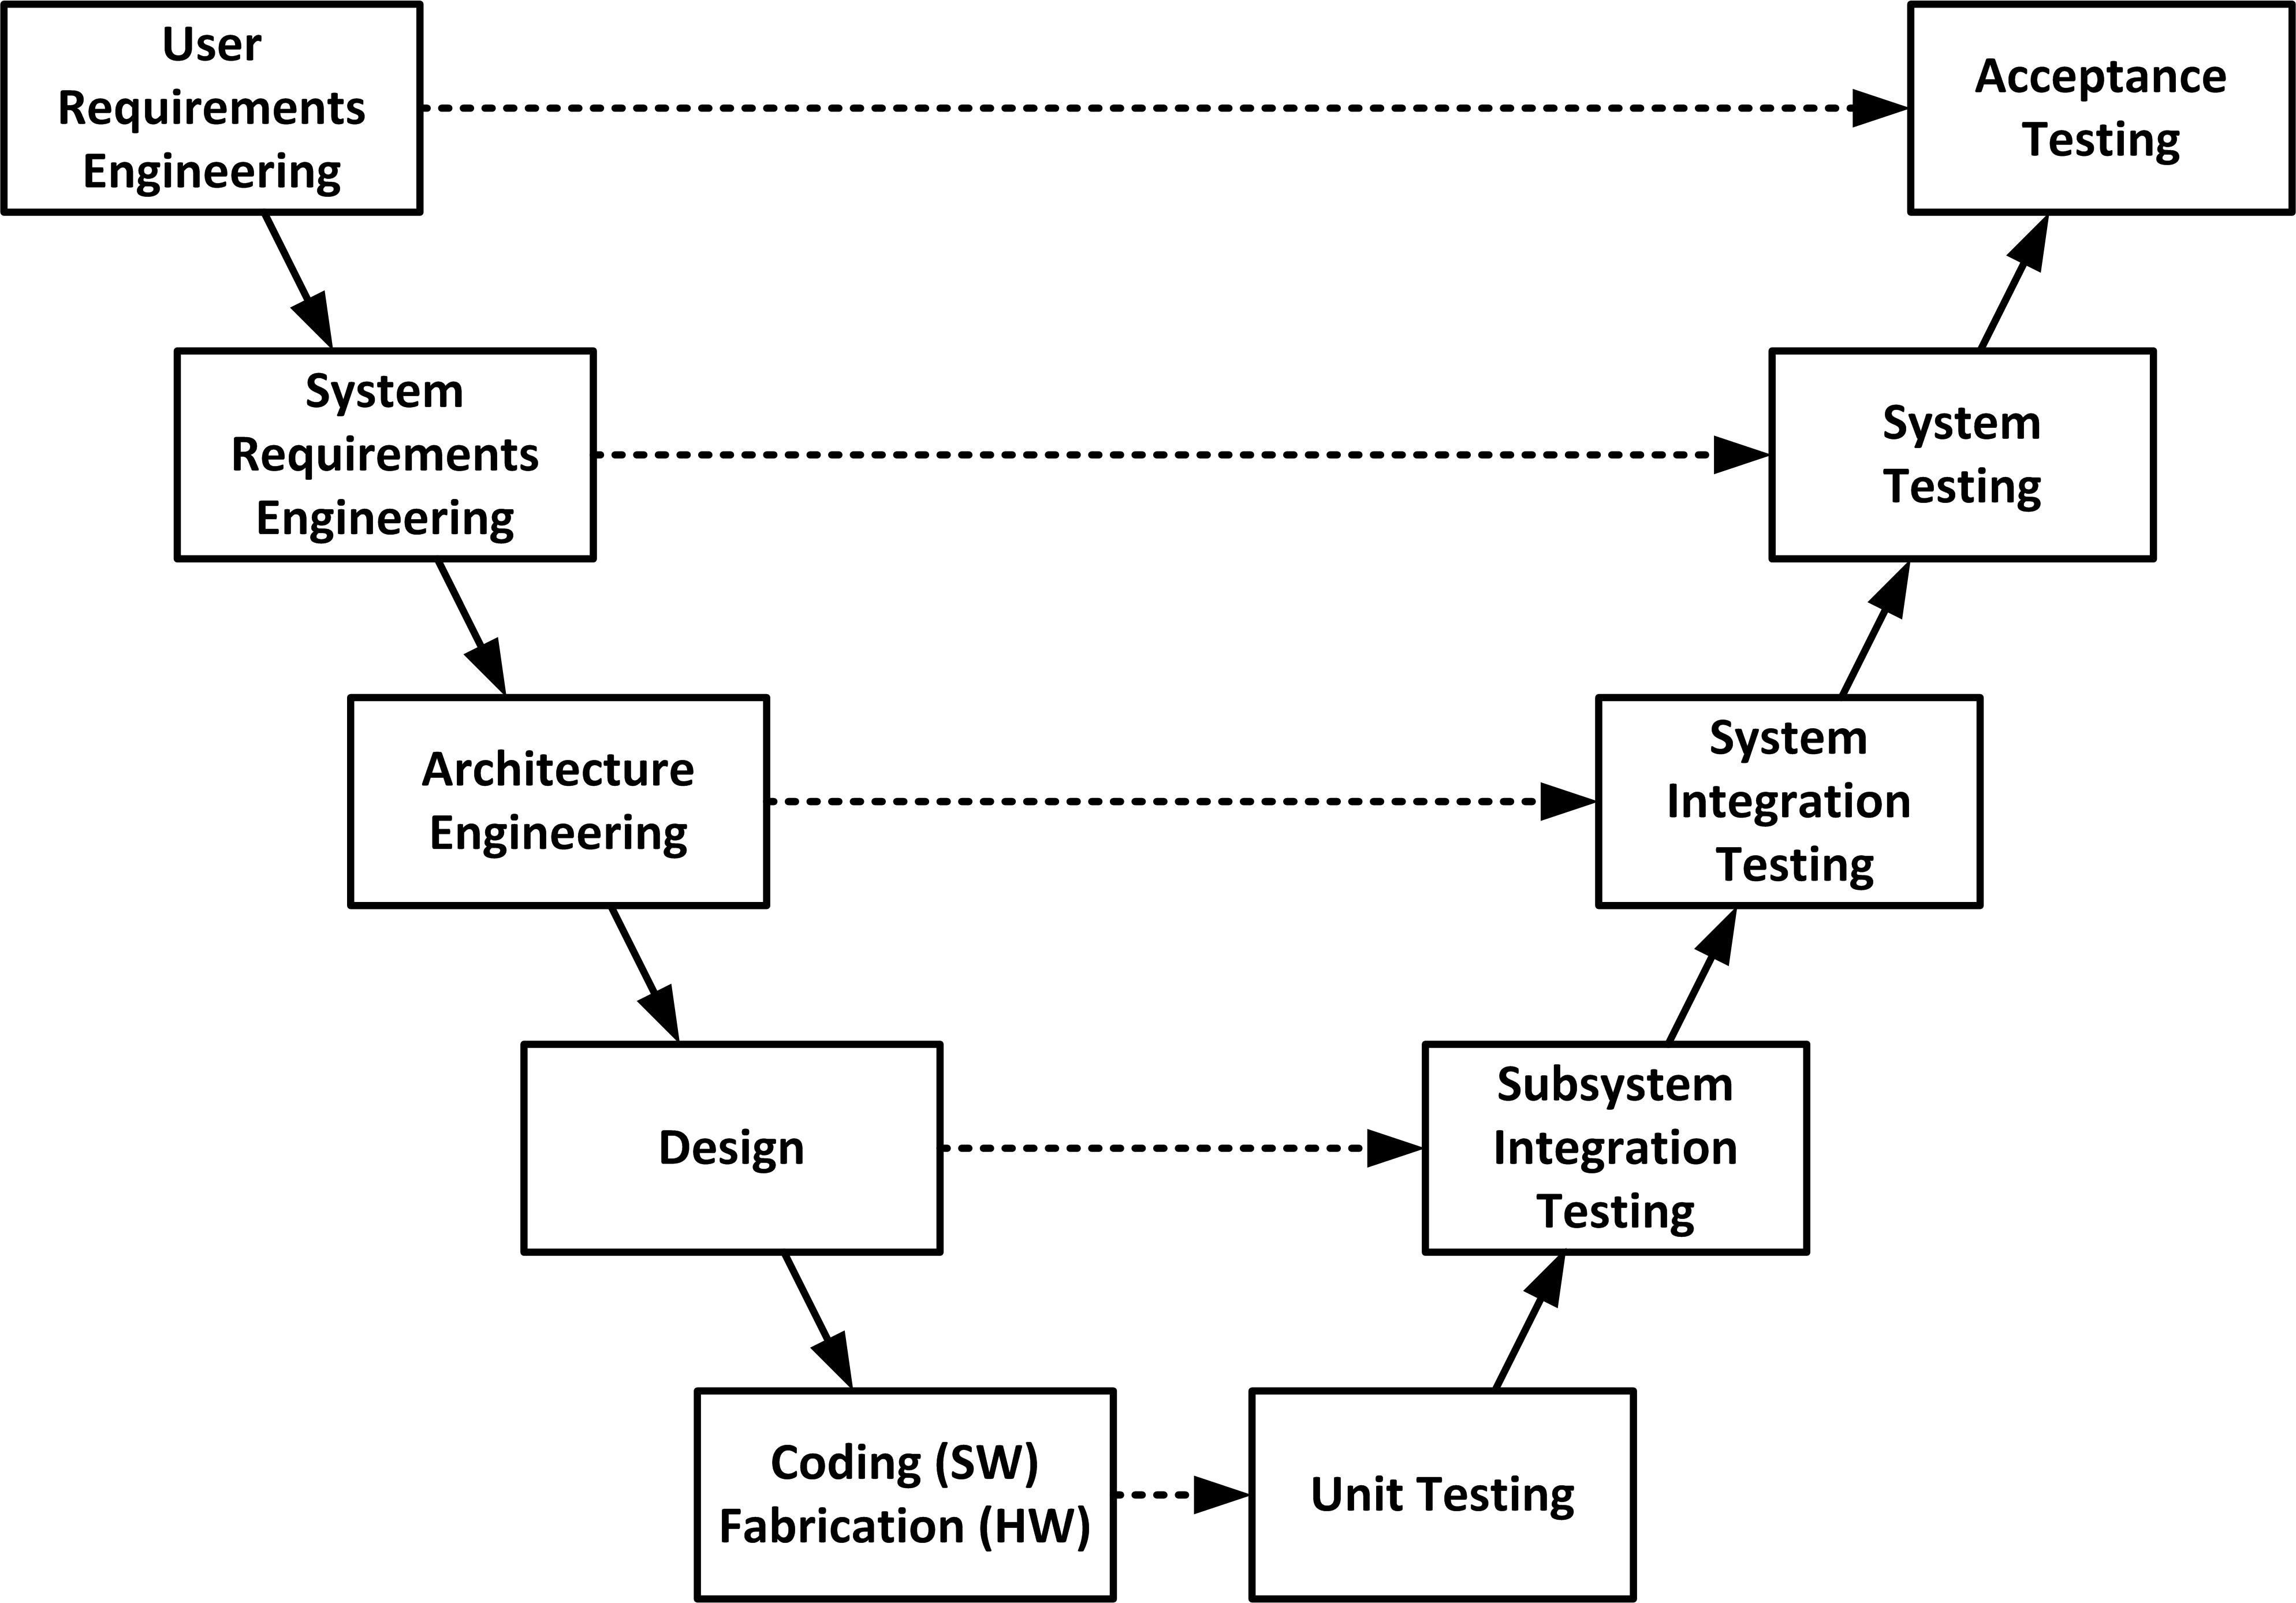
\includegraphics[width=.5\linewidth]{V}
       
    \end{block}
    \begin{block}{\large Various phases of the V-model }
        \centering
        \begin{itemize}
            \item \textbf{ Requirements} like BRS and SRS begin the life cycle model just like the waterfall model. But, in this model before development is started, a system test plan is created.  The test plan focuses on meeting the functionality specified in the requirements gathering.

            \item \textbf{ The high-level design (HLD) phase} focuses on system architecture and design. It provide overview of solution, platform, system, product and service/process. An integration test plan is created in this phase as well in order to test the pieces of the software systems ability to work together.
            
            \item \textbf{ The low-level design (LLD) phase} is where the actual software components are designed. It defines the actual logic for each and every component of the system. Class diagram with all the methods and relation between classes comes under LLD. Component tests are created in this phase as well.
            
            \item \textbf{ The implementation phase} is, again, where all coding takes place. Once coding is complete, the path of execution continues up the right side of the V where the test plans developed earlier are now put to use.
            
            \item \textbf{ The coding phase} is at the bottom of the V-Shape model. Module design is converted into code by developers. Unit Testing is performed by the developers on the code written by them.
        \end{itemize}
    \end{block}  
     \begin{block}{\large When to use V-Shaped Model}
        \centering
        \begin{itemize}
            \item The V-shaped model should be used for small to medium sized projects where requirements are clearly defined and fixed.
            \item The V-Shaped model should be chosen when ample technical resources are available with needed technical expertise.
        \end{itemize}
    \end{block}  
    \begin{columns}[t]
      \begin{column}{.48\linewidth}
        \begin{block}{Advantages}
          \begin{itemize}
          \item Simple and easy to use.
          \item Each phase has specific deliverables.
          \item Higher chance of success over the waterfall model
                due to the early development of test plans during the
                life cycle.
          \item Works well for small projects where requirements are
                easily understood.
          \end{itemize}
        \end{block}
      \end{column}
      \begin{column}{.48\linewidth}
        \begin{block}{Disadvantages}
          \begin{itemize}
          \item Very rigid like the waterfall model.
          \item Little flexibility and adjusting scope is difficult and
                expensive.
          \item Software is developed during the implementation phase,
                so no early prototypes of the software are produced.
          \item This Model does not provide a clear path for problems
                found during testing phases
          \end{itemize}
        \end{block}
      \end{column}
    \end{columns}
  \end{frame}
  \begin{frame}{Agile Development}
  \begin{block}{\large The Four Values of The Agile Manifesto}

        The Agile Manifesto is comprised of four foundational values and 12 supporting principles which lead the Agile approach to software development. Each Agile methodology applies the four values in different ways, but all of them rely on them to guide the development and delivery of high-quality, working software.
        \begin{itemize}
            \item \textbf{Individuals and Interactions} over \textbf{Processes and Tools}
            
            \item \textbf{Working Software} over \textbf{Comprehensive Documentation}
            
            \item \textbf{Customer Collaboration} over \textbf{Contract Negotiation}
            
            
            \item \textbf{Responding to Change} over \textbf{Following a Plan }
            
        \end{itemize}
        \textit{That is, while there is value in the items on
        the right, we value the items on the left more.}
    \end{block}  
     \begin{block}{\large The twelve principles of agile development}
         \begin{columns}[t]
      \begin{column}{.48\linewidth}
            \begin{itemize}
                \item \textbf{Customer satisfaction through early and continuous software delivery –} Customers are happier when they receive working software at regular intervals, rather than waiting extended periods of time between releases.
                \item \textbf{Accommodate changing requirements throughout the development process – }The ability to avoid delays when a requirement or feature request changes.
                \item \textbf{Frequent delivery of working software – }Scrum accommodates this principle since the team operates in software sprints or iterations that ensure regular delivery of working software.
                \item \textbf{Collaboration between the business stakeholders and developers throughout the project –} Better decisions are made when the business and technical team are aligned.
                \item \textbf{Support, trust, and motivate the people involved –} Motivated teams are more likely to deliver their best work than unhappy teams.
                \item \textbf{Enable face-to-face interactions –} Communication is more successful when development teams are co-located.
            \end{itemize}
            \end{column}
        \begin{column}{.48\linewidth}
            \begin{itemize}
                \item \textbf{Working software is the primary measure of progress –} Delivering functional software to the customer is the ultimate factor that measures progress.
                \item \textbf{Agile processes to support a consistent development pace –} Teams establish a repeatable and maintainable speed at which they can deliver working software, and they repeat it with each release.
                \item \textbf{Attention to technical detail and design enhances agility – } The right skills and good design ensures the team can maintain the pace, constantly improve the product, and sustain change.
                \item \textbf{Simplicity – }Develop just enough to get the job done for right now.
                \item \textbf{Self-organizing teams encourage great architectures, requirements, and designs –} Skilled and motivated team members who have decision-making power, take ownership, communicate regularly with other team members, and share ideas that deliver quality products.
                \item \textbf{Regular reflections on how to become more effective –} Self-improvement, process improvement, advancing skills, and techniques help team members work more efficiently.
            \end{itemize}
        \end{column}
    \end{columns}
    \end{block}
     \begin{block}{\large Scrum Team}
      \centering
        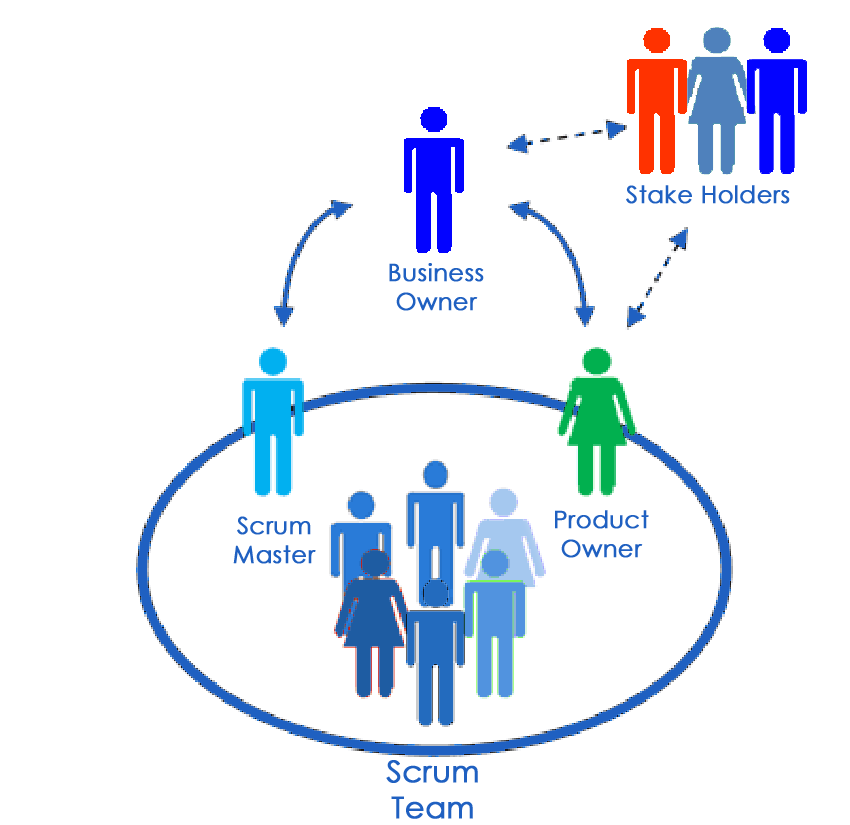
\includegraphics[width=.3\linewidth]{scrum}
    \end{block}  
     \begin{block}{Scrum overview}  
    \begin{columns}[t]
      \begin{column}{.48\linewidth}
        
          \begin{itemize}
                \item A product owner creates a prioritized wish list called a product backlog.
                \item During sprint planning, the team pulls a small chunk from the top of that wish list, a sprint backlog, and decides how to implement those pieces.
                \item The team has a certain amount of time — a sprint (usually two to four weeks) — to complete its work, but it meets each day to assess its progress (daily Scrum).
          \end{itemize}
      \end{column}
      \begin{column}{.48\linewidth}

          \begin{itemize}
                \item Along the way, the Scrum Master keeps the team focused on its goal.
                \item At the end of the sprint, the work should be potentially shippable: ready to hand to a customer, put on a store shelf, or show to a stakeholder.
                \item The sprint ends with a sprint review and retrospective.
                \item As the next sprint begins, the team chooses another chunk of the product backlog and begins working again

          \end{itemize}
      
      \end{column}
    \end{columns}
      \end{block}
  \end{frame}
%%%%%%%%%%%%%%%%%%%%%%%%%Core Concepts%%%%%%%%%%%%%%%%%%%%%%%%%%%%%%%%%  
  \begin{frame}{Core Concepts}
    \begin{columns}[t]
      \begin{column}{.48\linewidth}
        \begin{block}{Feature Driven Development (FDD)}
            Feature Driven Development (FDD) aims to minimise the number of processes to optimise a project's scalability and repeatability. The core principles are as follows: 
            \begin{itemize}
                \item A system for building systems is necessary in order to scale to larger projects.
                \item A simple, but well-define process will work best.
                \item Process steps should be logical and their worth immediately obvious to each team member.
                \item "Process pride" can keep the real work from happening.
                \item Good processes move to the background so team members can focus on results.
                \item Short, iterative, feature-driven life cycles are best.
            \end{itemize}
            FDD recommends the follow time scales to develop products:  
            \begin{itemize}
                \item Develop an overall model (10\% initial, 4\%  ongoing)
                \item Build a features list (4\%  initial, 1\%  ongoing)
                \item Plan by feature (2\%  initial, 2\%  ongoing)
                \item Design by feature
                \item Build by feature (77\% for design and build combined)
            \end{itemize}
        \end{block}
        \begin{block}{Joint Application Development (JAD)}
            JAD is a requirements-definition and user-interface design methodology in which end-users, executives, and developers attend intense off-site meetings to work out a system's details. So the Joint Application Development (JAD) methodology aims to involve the client in the design and development of an application. This is accomplished through a series of collaborative workshops called JAD sessions.
     
            JAD focuses on the business problem rather than technical details. It is most applicable to the development of business systems, but it can be used successfully for systems software. It produces its savings by shortening the elapsed time required to gather a system's requirements and by gathering requirements better, thus reducing the number of costly, downstream requirements changes. Its success depends on effective leadership of the JAD sessions; on participation by key end-users, executives, and developers; and on achieving group synergy during JAD sessions.
             
            In contrast to the Waterfall approach, JAD is thought to lead to shorter development times and greater client satisfaction, both of which stem from the constant involvement of the client throughout the development process. On the other hand, with the traditional approach to systems development, the developer investigates the system requirements and develops an application, with client input consisting of a series of interviews.
             

        \end{block}
        \begin{block}{Rapid Application Development (RAD)}
           Rapid-Development Languages (RDLs) produce their savings by reducing the amount of construction needed to build a product. Although the savings are realized during construction, the ability to shorten the construction cycle has project wide implications: shorter construction cycles make incremental life cycles such as Evolutionary Prototyping practical. Because RDLs often lack first-rate performance, constrain flexibility, and are limited to specific kinds of problems, they are usually better suited to the development of in-house business software and limited-distribution custom software than systems software.
 
            The RAD proposes that products can be developed faster and of higher quality by:
            \begin{itemize}
                \item Using workshops or focus groups to gather requirements.
                \item Prototyping and user testing of designs.
                \item Re-using software components.
                \item Following a schedule that defers design improvements to the next product version.
                \item Keeping review meetings and other team communication informal.
            \end{itemize}
            

        \end{block}
      \end{column}
      \begin{column}{.48\linewidth}
        \begin{block}{Rational Unified Process (RUP) }
            The Rational Unified Process attempts to capture many of modern software development's best practices in a form suitable for a wide range of projects and organizations. This process recognizes that the traditional waterfall approach can be inefficient because it idles key team members for extended periods of time. Many feel that the waterfall approach also introduces a lot of risk because it defers testing and integration until the end of the project lifecycle. Problems found at this stage are very expense to fix.
 
            By contrast, RUP represents an iterative approach that is superior for a number of reasons:
            \begin{itemize}
                \item It lets you take into account changing requirements which despite the best efforts of all project managers are still a reality on just about every project.
                \item Integration is not one big bang at the end; instead, elements are integrated progressively.
                \item Risks are usually discovered or addressed during integration. With the iterative approach, you can mitigate risks earlier.
                \item Iterative development provides management with a means of making tactical changes to the product. It allows you to release a product early with reduced functionality to counter a move by a competitor, or to adopt another vendor for a given technology.
                \item Iteration facilitates reuse; it is easier to identify common parts as they are partially designed or implemented than to recognize them during planning.
                \item When you can correct errors over several iterations, the result is a more robust architecture. Performance bottlenecks are discovered at a time when they can still be addressed, instead of creating panic on the eve of delivery.
                \item Developers can learn along the way, and their various abilities and specialties are more fully employed during the entire lifecycle. Testers start testing early, technical writers begin writing early, and so on.
                \item The development process itself can be improved and refined along the way. The assessment at the end of iteration not only looks at the status of the project from a product or schedule perspective, but also analyzes what should be changed in the organization and in the process to make it perform better in the next iteration.
 
            \end{itemize}
            

        \end{block}
        \begin{block}{Scrum}
                Scrum is characterized by:
                \begin{itemize}
                \item A living backlog of prioritized work to be done.
                \item Completion of a largely fixed set of backlog items in a series of short iterations or sprints.
                \item A brief daily meeting (called a scrum), at which progress is explained, upcoming work is described, and obstacles are raised.
                \item A brief planning session in which the backlog items for the sprint will be defined.
                \item A brief heartbeat retrospective, at which all team members reflect about the past sprint.
                \end{itemize}
                Scrum is facilitated by a scrum master, whose primary job is to remove impediments to the ability of the team to deliver the sprint goal. The scrum master is not the leader of the team (as they are self-organizing) but acts as a productivity buffer between the team and any destabilizing influences.
         
                Scrum enables the creation of self-organizing teams by encouraging verbal communication across all team members and across all disciplines that are involved in the project. A key principle of scrum is its recognition that fundamentally empirical challenges cannot be addressed successfully in a traditional "process control" manner. As such, scrum adopts an empirical approach - accepting that the problem cannot be fully understood or defined, focusing instead on maximizing the team's ability to respond in an agile manner to emerging challenges.
        \end{block}
      \end{column}
    \end{columns}
  \end{frame}
  
\end{document}


%%%%%%%%%%%%%%%%%%%%%%%%%%%%%%%%%%%%%%%%%%%%%%%%%%%%%%%%%%%%%%%%%%%%%%%%%%%%%%%%%%%%%%%%%%%%%%%%%%%%
%%% Local Variables: 
%%% mode: latex
%%% TeX-PDF-mode: t
%%% End:
